\documentclass[aspectratio=169,10pt]{beamer}
\usetheme{Madrid}
\usecolortheme{default}

\usepackage{hyperref}
\usepackage{tikz}
\usetikzlibrary{positioning,shapes.geometric,arrows.meta,calc}
\usepackage{circuitikz}
\usepackage{amsmath,amssymb}
\usepackage{listings}
\lstdefinestyle{juliastyle}{language=Julia,basicstyle=\ttfamily\tiny,keywordstyle=\bfseries\color{unibblue},commentstyle=\color{gray}\itshape,stringstyle=\color{unibgreen},backgroundcolor=\color{softgray},frame=single,rulecolor=\color{unibblue!30},breaklines=true,breakatwhitespace=true,showstringspaces=false,tabsize=2,numbers=none}
\usepackage{booktabs}

% --- Custom Colors ---
\definecolor{unibblue}{RGB}{0, 32, 96}
\definecolor{unibgold}{RGB}{197, 160, 89}
\definecolor{unibgreen}{RGB}{34, 112, 60}
\definecolor{softgray}{RGB}{245, 247, 250}

\setbeamercolor{palette primary}{bg=unibblue,fg=white}
\setbeamercolor{palette secondary}{bg=unibblue!85,fg=white}
\setbeamercolor{palette tertiary}{bg=unibblue!70,fg=white}
\setbeamercolor{structure}{fg=unibblue}
\setbeamercolor{titlelike}{parent=structure,bg=unibblue,fg=white}
\setbeamercolor{block title}{bg=unibblue!90,fg=white}
\setbeamercolor{block body}{bg=unibblue!8,fg=black}
\setbeamercolor{alertblock title}{bg=unibgold!95,fg=black}
\setbeamercolor{alertblock body}{bg=unibgold!15,fg=black}
\setbeamercolor{exampleblock title}{bg=unibgreen!90,fg=white}
\setbeamercolor{exampleblock body}{bg=unibgreen!10,fg=black}

% Listings setup for Julia
\lstdefinelanguage{Julia}{
  keywords={abstract,break,case,catch,const,continue,do,else,elseif,end,export,false,for,function,global,if,import,let,local,macro,module,mutable,primitive,quote,return,struct,true,try,type,using,var,while},
  sensitive=true,
  comment=[l]{\#},
  string=[b]"
}
\lstset{
  language=Julia,
  basicstyle=\ttfamily\tiny,
  keywordstyle=\color{blue!80!black}\bfseries,
  commentstyle=\color{green!50!black}\itshape,
  stringstyle=\color{red!80!black},
  breaklines=true,
  numbers=none,
  frame=single,
  backgroundcolor=\color{gray!5},
  aboveskip=2pt,
  belowskip=2pt
}

\title[Persamaan Diferensial (Minggu 13)]{Persamaan Diferensial}
\subtitle{Minggu 13: Persamaan Laplace 2D \& Elektrostatika: Sifat Harmonik, Beda Hingga FDM, dan Stres Isolator 150 kV IEC 60060-1}
\author[Novalio \& Arfan (UNIB)]{Ir. Novalio Daratha, S.T., M.Sc., Ph.D. \& Muhammad Arfan, S.T., M.T.}
\institute[Teknik Elektro UNIB]{Program Studi S1 Teknik Elektro, Jurusan Teknik Elektro \& Informatika\\Fakultas Teknik, Universitas Bengkulu}
\date[2026]{Semester Genap 2026}

\begin{document}

% -------------------------------------------------------------
% FRAME 1: Title Frame
% -------------------------------------------------------------
\begin{frame}[plain]
  \titlepage
\end{frame}

% -------------------------------------------------------------
% FRAME 2: Sub-CPMK OBE Bloom Taxonomy C1-C6
% -------------------------------------------------------------
\begin{frame}{Sub-CPMK Taksonomi Bloom (Minggu 13)}
  \begin{block}{Sub-Capaian Pembelajaran Mata Kuliah (Sub-CPMK 6)}
    Setelah menyelesaikan pembelajaran pada modul Minggu 13 ini, mahasiswa mampu:
    \begin{itemize}
      \item \textbf{C1 (Mengingat):} Menyatakan bentuk baku Persamaan Laplace 2D ($\nabla^2 V = 0$) dan hubungan medan potensial $\vec{E} = -\nabla V$.
      \item \textbf{C2 (Memahami):} Menjelaskan Teorema Nilai Rata-rata Gauss dan Prinsip Ekstremum (tanpa titik puncak lokal di ruang bebas).
      \item \textbf{C3 (Menerapkan):} Menurunkan solusi potensial analitis $V(x,y)$ pada palung konduktor berbatas pelat bertegangan.
      \item \textbf{C4 (Menganalisis):} Menghitung vektor intensitas medan listrik $\vec{E}$ dan mengidentifikasi konsentrasi stres dielektrik.
      \item \textbf{C5 (Mengevaluasi):} Mengevaluasi batas medan kritis korona Peek ($\approx 30\text{ kV/cm}$) pada rantai isolator SUTT 150 kV PLN.
      \item \textbf{C6 (Menciptakan/Komputasi):} Mengembangkan simulasi beda hingga (FDM) relaksasi SOR pada bahasa ilmiah \textbf{Julia}.
    \end{itemize}
  \end{block}
\end{frame}

% -------------------------------------------------------------
% FRAME 3: Peta Kurikulum & Transisi ke PDP Elliptik
% -------------------------------------------------------------
\begin{frame}{Peta Kurikulum: Medan Elektrostatik dalam Kesetimbangan}
  \begin{columns}[t]
    \begin{column}{0.48\textwidth}
      \begin{block}{Karakteristik PDP Elliptik ($\Delta < 0$)}
        \small
        \begin{itemize}
          \item Berbeda dari gelombang ($u_{tt}$) dan difusi ($u_t$), Persamaan Laplace \textbf{tidak bergantung waktu}: $\partial/\partial t = 0$.
          \item Mengatur kesetimbangan statis medan potensial dalam ruang tertutup.
          \item Nilai di setiap titik ruang terikat kokoh oleh kondisi seluruh batas kelilingnya (\textit{boundary-driven}).
        \end{itemize}
      \end{block}
    \end{column}
    \begin{column}{0.48\textwidth}
      \begin{alertblock}{Relevansi Rekayasa Tegangan Tinggi}
        \small
        \begin{itemize}
          \item Perancangan isolator porselen/polimer GITET 500 kV.
          \item Distribusi medan kabel daya XLPE \& terminasi sambungan.
          \item Mencegah konsentrasi stres medan yang memicu \textit{partial discharge} dan tembus listrik (\textit{dielectric breakdown}).
        \end{itemize}
      \end{alertblock}
    \end{column}
  \end{columns}
  \vspace{0.05cm}
  \begin{exampleblock}{Persamaan Laplace \& Poisson Skalar 2D}
    \small
    Ruang tanpa muatan bebas: $\nabla^2 V = \frac{\partial^2 V}{\partial x^2} + \frac{\partial^2 V}{\partial y^2} = 0$. \quad Ada muatan bebas: $\nabla^2 V = -\frac{\rho_v}{\epsilon}$.
  \end{exampleblock}
\end{frame}

% -------------------------------------------------------------
% FRAME 4: Dari Hukum Gauss ke Persamaan Laplace
% -------------------------------------------------------------
\begin{frame}{Penurunan Matematis dari Hukum Gauss Elektrostatika}
  Berdasarkan dua postulat medan elektrostatik dasar dalam media homogen isotropik ($\epsilon$ konstan):
  \vspace{0.1cm}
  \begin{columns}[t]
    \begin{column}{0.48\textwidth}
      \begin{block}{1. Hukum Gauss Diferensial}
        \small
        Divergensi kerapatan fluks medan listrik sama dengan kerapatan muatan volume:
        \begin{equation*}
          \nabla \cdot \vec{D} = \rho_v \implies \nabla \cdot \vec{E} = \frac{\rho_v}{\epsilon}
        \end{equation*}
      \end{block}
      \begin{alertblock}{2. Hubungan Medan-Potensial}
        \small
        Karena medan elektrostatik bersifat konservatif ($\nabla \times \vec{E} = 0$), medan adalah minus gradien potensial skalar:
        \begin{equation*}
          \mathbf{\vec{E} = -\nabla V = -\left( \frac{\partial V}{\partial x}\hat{a}_x + \frac{\partial V}{\partial y}\hat{a}_y \right)}
        \end{equation*}
      \end{alertblock}
    \end{column}
    \begin{column}{0.48\textwidth}
      \begin{exampleblock}{3. Substitusi Menghasilkan Laplace}
        \small
        Substitusikan $\vec{E} = -\nabla V$ ke Hukum Gauss:
        \begin{equation*}
          \nabla \cdot (-\nabla V) = \frac{\rho_v}{\epsilon} \implies \mathbf{\nabla^2 V = -\frac{\rho_v}{\epsilon}}
        \end{equation*}
        Di dalam media dielektrik murni tanpa muatan bebas ($\rho_v = 0$):
        \begin{equation*}
          \mathbf{\nabla^2 V = \frac{\partial^2 V}{\partial x^2} + \frac{\partial^2 V}{\partial y^2} = 0}
        \end{equation*}
      \end{exampleblock}
    \end{column}
  \end{columns}
\end{frame}

% -------------------------------------------------------------
% FRAME 5: Sifat Fundamental Fungsi Harmonik
% -------------------------------------------------------------
\begin{frame}{Sifat Fundamental Fungsi Harmonik: Nilai Rata-rata \& Ekstremum}
  Setiap solusi yang memenuhi Persamaan Laplace disebut sebagai \textbf{Fungsi Harmonik}:
  \vspace{0.1cm}
  \begin{columns}[t]
    \begin{column}{0.48\textwidth}
      \begin{block}{Teorema Nilai Rata-rata Gauss}
        \small
        Potensial di sembarang titik $(x_0, y_0)$ tepat sama dengan rata-rata potensial pada lingkaran konsentris berjari-jari $R$ di sekitarnya:
        \begin{equation*}
          \mathbf{V(x_0, y_0) = \frac{1}{2\pi R} \oint_{\mathcal{C}} V \, ds}
        \end{equation*}
        \textbf{Konsekuensi:} Tidak ada muatan yang dapat terperangkap di titik tunggal media tanpa elektroda.
      \end{block}
    \end{column}
    \begin{column}{0.48\textwidth}
      \begin{alertblock}{Prinsip Maksimum-Minimum}
        \small
        Fungsi harmonik \textbf{tidak pernah} memiliki nilai ekstremum lokal (puncak atau lembah) di dalam interior domain:
        \begin{itemize}
          \item Nilai potensial maksimum mutlak dan minimum mutlak \textbf{pasti terletak pada batas elektroda}!
          \item Jika seluruh batas ditanahkan ($V = 0$), maka seluruh interior pasti bernilai nol identik.
        \end{itemize}
      \end{alertblock}
    \end{column}
  \end{columns}
\end{frame}

% -------------------------------------------------------------
% FRAME 6: Teorema Ketunggalan & Vektor Medan Listrik
% -------------------------------------------------------------
\begin{frame}{Teorema Ketunggalan (\textit{Uniqueness}) \& Vektor Medan}
  \begin{columns}[t]
    \begin{column}{0.52\textwidth}
      \begin{block}{Teorema Ketunggalan Medan (Uniqueness)}
        \small
        Jika suatu fungsi potensial $V(x, y)$ memenuhi Persamaan Laplace pada seluruh ruang $\Omega$ dan memenuhi syarat batas pada keliling $\partial \Omega$, maka $V(x, y)$ adalah \textbf{satu-satunya solusi yang eksis}:
        \begin{itemize}
          \item Metode apa pun yang digunakan (analitis deret Fourier, beda hingga numerik FDM, atau konformal) pasti konvergen ke solusi fisik yang identik!
        \end{itemize}
      \end{block}
    \end{column}
    \begin{column}{0.44\textwidth}
      \begin{alertblock}{Fluks Listrik \& Garis Ekuipotensial}
        \small
        \begin{itemize}
          \item Vektor medan listrik $\vec{E}$ selalu tegak lurus ($90^\circ$) terhadap garis kontur ekuipotensial.
          \item Permukaan konduktor adalah permukaan ekuipotensial sempurna.
          \item Rapat muatan permukaan konduktor:
          \begin{equation*}
            \rho_s = \epsilon E_n = -\epsilon \left.\frac{\partial V}{\partial n}\right|_{\text{permukaan}}
          \end{equation*}
        \end{itemize}
      \end{alertblock}
    \end{column}
  \end{columns}
\end{frame}

% -------------------------------------------------------------
% FRAME 7: Diskritisasi FDM Stensil 5-Titik & Gauss-Seidel
% -------------------------------------------------------------
\begin{frame}{Metode Beda Hingga (FDM) \& Relaksasi Gauss-Seidel / SOR}
  Turunan kedua didekati dengan beda hingga terpusat orde 2 ($\Delta x = \Delta y = h$):
  \begin{equation*}
    \frac{\partial^2 V}{\partial x^2} \approx \frac{V_{i+1,j} - 2V_{i,j} + V_{i-1,j}}{h^2}, \quad \frac{\partial^2 V}{\partial y^2} \approx \frac{V_{i,j+1} - 2V_{i,j} + V_{i,j-1}}{h^2}
  \end{equation*}
  \begin{columns}[t]
    \begin{column}{0.48\textwidth}
      \begin{block}{Stensil 5-Titik Laplace}
        \small
        Jumlahkan kedua turunan dan samakan dengan nol:
        \begin{equation*}
          \mathbf{V_{i,j} = \frac{1}{4}\left( V_{i+1,j} + V_{i-1,j} + V_{i,j+1} + V_{i,j-1} \right)}
        \end{equation*}
        Potensial tiap titik adalah rata-rata dari 4 tetangganya!
      \end{block}
    \end{column}
    \begin{column}{0.48\textwidth}
      \begin{alertblock}{Pembaruan Terakselerasi SOR}
        \small
        Untuk percepatan konvergensi ($\omega \in [1, 2]$):
        \begin{equation*}
          V_{i,j}^{(k+1)} = (1-\omega)V_{i,j}^{(k)} + \frac{\omega}{4}\left( V_{i+1,j}^{(k)} + V_{i-1,j}^{(k+1)} + \dots \right)
        \end{equation*}
        Iterasi berhenti jika $\max |V^{(k+1)} - V^{(k)}| < \epsilon_{\text{tol}}$.
      \end{alertblock}
    \end{column}
  \end{columns}
\end{frame}

% -------------------------------------------------------------
% FRAME 8: Diagram Palung Konduktor 2D
% -------------------------------------------------------------
\begin{frame}{Geometri Palung Konduktor \& Garis Ekuipotensial 2D}
  \begin{columns}[t]
    \begin{column}{0.48\textwidth}
      \begin{block}{Palung Logam Bujur Sangkar ($1\text{ m} \times 1\text{ m}$)}
        \centering
        \resizebox{\linewidth}{!}{%
        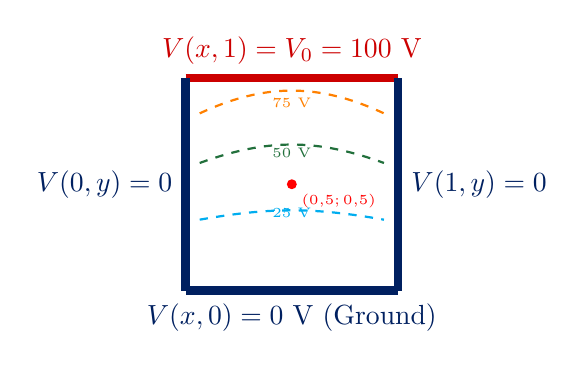
\begin{tikzpicture}[scale=0.9]
          % Electrodes
          \draw[line width=3pt, red!80!black] (0, 3) -- (3, 3) node[midway, above] {$V(x, 1) = V_0 = 100\text{ V}$};
          \draw[line width=3pt, unibblue] (0, 0) -- (3, 0) node[midway, below] {$V(x, 0) = 0\text{ V (Ground)}$};
          \draw[line width=3pt, unibblue] (0, 0) -- (0, 3) node[midway, left] {$V(0, y) = 0$};
          \draw[line width=3pt, unibblue] (3, 0) -- (3, 3) node[midway, right] {$V(1, y) = 0$};
          % Equipotential curves
          \draw[thick, dashed, orange] (0.2, 2.5) to[bend left=25] (2.8, 2.5);
          \node[orange, font=\tiny] at (1.5, 2.65) {$75\text{ V}$};
          \draw[thick, dashed, unibgreen] (0.2, 1.8) to[bend left=20] (2.8, 1.8);
          \node[unibgreen, font=\tiny] at (1.5, 1.95) {$50\text{ V}$};
          \draw[thick, dashed, cyan] (0.2, 1.0) to[bend left=10] (2.8, 1.0);
          \node[cyan, font=\tiny] at (1.5, 1.1) {$25\text{ V}$};
          \fill[red] (1.5, 1.5) circle (2pt) node[below right, font=\tiny] {$(0{,}5; 0{,}5)$};
        \end{tikzpicture}
        }
      \end{block}
    \end{column}
    \begin{column}{0.48\textwidth}
      \begin{alertblock}{Solusi Analitis Deret Fourier}
        \small
        Pemisahan variabel $V(x, y) = X(x) Y(y)$:
        \begin{equation*}
          V(x, y) = \frac{4V_0}{\pi} \sum_{k=1}^{\infty} \frac{\sin((2k-1)\pi x) \sinh((2k-1)\pi y)}{(2k-1) \sinh((2k-1)\pi)}
        \end{equation*}
        \textbf{Wawasan Fisika:}
        Fungsi $\sinh(y)$ melonjak curam di dekat pelat atas, menciptakan gradien medan listrik terkuat di sekitar sudut $y = 1\text{ m}$.
      \end{alertblock}
    \end{column}
  \end{columns}
\end{frame}

% -------------------------------------------------------------
% FRAME 9: Contoh Soal Terhitung Langkah demi Langkah
% -------------------------------------------------------------
\begin{frame}{Contoh Terhitung: Evaluasi Potensial di Titik Pusat Palung}
  \begin{exampleblock}{Masalah: Palung konduktor $a = b = 1\text{ m}$ dengan $V_0 = 100\text{ V}$ di atap dan 3 dinding ground}
    Hitung nilai potensial di titik tengah $(x = 0{,}5; y = 0{,}5)$ menggunakan deret Fourier dan verifikasi teorema simetri!
  \end{exampleblock}
  \begin{columns}[t]
    \begin{column}{0.48\textwidth}
      \begin{block}{Evaluasi Suku Pertama \& Kedua}
        \small
        \textbf{1. Suku Pertama ($k=1 \implies n=1$):}
        \begin{align*}
          V_1 &= \frac{400}{\pi} \frac{\sinh(\pi/2)}{\sinh(\pi)} \sin\left(\frac{\pi}{2}\right) \\
              &= 127{,}32 \times \frac{2{,}3013}{11{,}5487} \times 1 \approx \mathbf{25{,}37\text{ V}}
        \end{align*}
        \textbf{2. Suku Kedua ($n=3$):}
        $V_3 = \frac{400}{3\pi} \frac{\sinh(3\pi/2)}{\sinh(3\pi)} (-1) \approx \mathbf{-0{,}38\text{ V}}$.
      \end{block}
    \end{column}
    \begin{column}{0.48\textwidth}
      \begin{alertblock}{Superposisi \& Verifikasi Simetri}
        \small
        \textbf{3. Superposisi Analitis:}
        \begin{equation*}
          V(0{,}5; 0{,}5) \approx V_1 + V_3 = 25{,}37 - 0{,}38 = \mathbf{24{,}99\text{ V}}
        \end{equation*}
        \textbf{4. Teorema Rata-rata Simetri:}
        Oleh superposisi 4 sisi bujur sangkar:
        \begin{equation*}
          V_{\text{pusat}} = \frac{V_0 + 0 + 0 + 0}{4} = \frac{100}{4} = \mathbf{25{,}00\text{ V}} \quad \qed
        \end{equation*}
      \end{alertblock}
    \end{column}
  \end{columns}
\end{frame}

% -------------------------------------------------------------
% FRAME 10: Contoh Kasus Gradien Medan Listrik
% -------------------------------------------------------------
\begin{frame}{Contoh Terhitung: Intensitas Medan Listrik dari Gradien $\vec{E} = -\nabla V$}
  \begin{exampleblock}{Masalah: Distribusi potensial dielektrik $V(x, y) = 50(x^2 - y^2) + 20x$ [V]}
    1. Buktikan memenuhi Persamaan Laplace 2D! \quad 2. Hitung besar magnitudo $|\vec{E}|$ pada titik $(x = 2\text{ cm}, y = 1\text{ cm})$!
  \end{exampleblock}
  \begin{columns}[t]
    \begin{column}{0.48\textwidth}
      \begin{block}{1. Pembuktian Persamaan Laplace}
        \small
        Turunan parsial:
        $\frac{\partial V}{\partial x} = 100x + 20 \implies \frac{\partial^2 V}{\partial x^2} = +100$,\\
        $\frac{\partial V}{\partial y} = -100y \implies \frac{\partial^2 V}{\partial y^2} = -100$.\\[2pt]
        Jumlahkan:
        \begin{equation*}
          \nabla^2 V = 100 + (-100) = \mathbf{0} \quad \text{(Terbukti Laplace!)}
        \end{equation*}
      \end{block}
    \end{column}
    \begin{column}{0.48\textwidth}
      \begin{alertblock}{2. Perhitungan Medan $\vec{E} = -\nabla V$}
        \small
        Vektor intensitas medan listrik:
        \begin{equation*}
          \vec{E} = -(100x + 20)\hat{a}_x + 100y\hat{a}_y \quad \text{[V/m]}
        \end{equation*}
        Evaluasi pada $x = 0{,}02\text{ m}, y = 0{,}01\text{ m}$:
        $E_x = -22\text{ V/m}, \quad E_y = +1\text{ V/m}$.\\[2pt]
        Magnitudo medan total:
        \begin{equation*}
          |\vec{E}| = \sqrt{(-22)^2 + 1^2} = \sqrt{485} \approx \mathbf{22{,}02\text{ V/m}} \quad \qed
        \end{equation*}
      \end{alertblock}
    \end{column}
  \end{columns}
\end{frame}

% -------------------------------------------------------------
% FRAME 11: Stres Dielektrik Rantai Isolator 150 kV
% -------------------------------------------------------------
\begin{frame}{Stres Dielektrik Rantai Isolator 150 kV \& Kapasitansi Liar}
  \begin{block}{Distribusi Tegangan Tak Linier pada Rantai Isolator Piringan}
    \small
    Pada SUTT 150 kV ($V_{\text{fasa}} = 86{,}6\text{ kV}$), rantai 9--10 piringan tidak membagi tegangan sama rata akibat kapasitansi liar ke tiang tanah ($C_e$):
  \end{block}
  \begin{columns}[t]
    \begin{column}{0.48\textwidth}
      \begin{alertblock}{Konsentrasi Tegangan Terparah}
        \small
        \begin{itemize}
          \item \textbf{Piringan \#1 (Dekat Kawat Fasa):} Memikul hingga $\approx 25 - 30\%$ dari total tegangan fasa ($\sim 25\text{ kV}$).
          \item \textbf{Piringan Tengah:} Memikul porsi tegangan terendah ($\sim 5 - 8\%$).
          \item Bentuk kurva menyerupai fungsi hiperbolik $\cosh(k x)$ yang diturunkan dari Persamaan Laplace 1D diskret!
        \end{itemize}
      \end{alertblock}
    \end{column}
    \begin{column}{0.48\textwidth}
      \begin{exampleblock}{Dampak Kerusakan Isolator}
        \small
        \begin{itemize}
          \item Piringan terbawah mengalami penuaan termal \& stres dielektrik ekstrem.
          \item Jika gradien medan melampaui ambang batas, terjadi lucutan permukaan (\textit{flashover}) yang memadamkan transmisi.
          \item Perlunya pemasangan \textbf{Grading Ring} (Cincin Korona) untuk mendongkrak kapasitansi ke kawat.
        \end{itemize}
      \end{exampleblock}
    \end{column}
  \end{columns}
\end{frame}

% -------------------------------------------------------------
% FRAME 12: Standar Industri: Batas Korona Peek & IEC 60060-1
% -------------------------------------------------------------
\begin{frame}{Standar Industri: Regulasi Medan Korona IEC 60060-1 \& IEEE 4}
  \begin{block}{Batas Medan Kritis Ionisasi Udara Peek}
    \small
    Rumus empiris Peek untuk timbulnya pelepasan muatan korona pada konduktor silinder:
    \begin{equation*}
      \mathbf{E_c = 30\, m \cdot \delta \left( 1 + \frac{0{,}3}{\sqrt{\delta \cdot r}} \right)} \quad [\text{kV/cm}] \quad (E_c \approx 30\text{ kV/cm} = 3\text{ MV/m})
    \end{equation*}
  \end{block}
  \vspace{0.05cm}
  \begin{table}[h]
    \centering
    \scriptsize
    \begin{tabular}{lccc}
      \toprule
      \textbf{Peralatan Tegangan Tinggi} & \textbf{Stres Medan Izin} & \textbf{Gejala Kegagalan Korona} & \textbf{Solusi Standar IEC 60060} \\
      \midrule
      Kawat Konduktor SUTT 150 kV & $\le 18\text{ kV/cm}$ & Rugi daya mendesis \& gas ozon & Konduktor berkas (\textit{bundle conductor}) \\
      Pin Tutup Isolator Porselen & $\le 25\text{ kV/cm}$ & Lucutan pendaran ungu \& erosi & Pemasangan \textit{Grading Ring} (Cincin) \\
      Bushing Transformator Tenaga & $\le 30\text{ kV/cm}$ & \textit{Partial discharge} internal & Layar kapasitif perata gradien \\
      \bottomrule
    \end{tabular}
  \end{table}
  \begin{alertblock}{Mitigasi Standar PLN}
    Pemasangan cincin perata medan menurunkan stres medan piringan terbawah hingga $40\%$, menyeimbangkan distribusi potensial sesuai standar keandalan transmisi.
  \end{alertblock}
\end{frame}

% -------------------------------------------------------------
% FRAME 13: Simulasi Komputasi Julia
% -------------------------------------------------------------
% FRAME 13: Praktikum Komputasi Julia
\begin{frame}[fragile]{Praktikum Komputasi Julia: FDM Laplace 2D Isolator}
  \begin{columns}[t]
    \column{0.50\textwidth}
    \begin{block}{Skrip Julia: Relaksasi Potensial 2D}
\begin{lstlisting}[style=juliastyle]
using Plots

Nx, Ny = 50, 50
V = zeros(Nx, Ny)
V[:, end] .= 150.0  # Batas atas 150 kV
V[:, 1] .= 0.0      # Batas tanah 0 V

# Iterasi Gauss-Seidel 5-Titik FDM
for it in 1:200, i in 2:Nx-1, j in 2:Ny-1
  V[i, j] = 0.25 * (V[i+1, j] + V[i-1, j] + V[i, j+1] + V[i, j-1])
end
contour(V, levels=12, color=:viridis)
\end{lstlisting}
    \end{block}

    \column{0.48\textwidth}
    \begin{alertblock}{Visualisasi Kontur Potensial 2D}
      \centering
      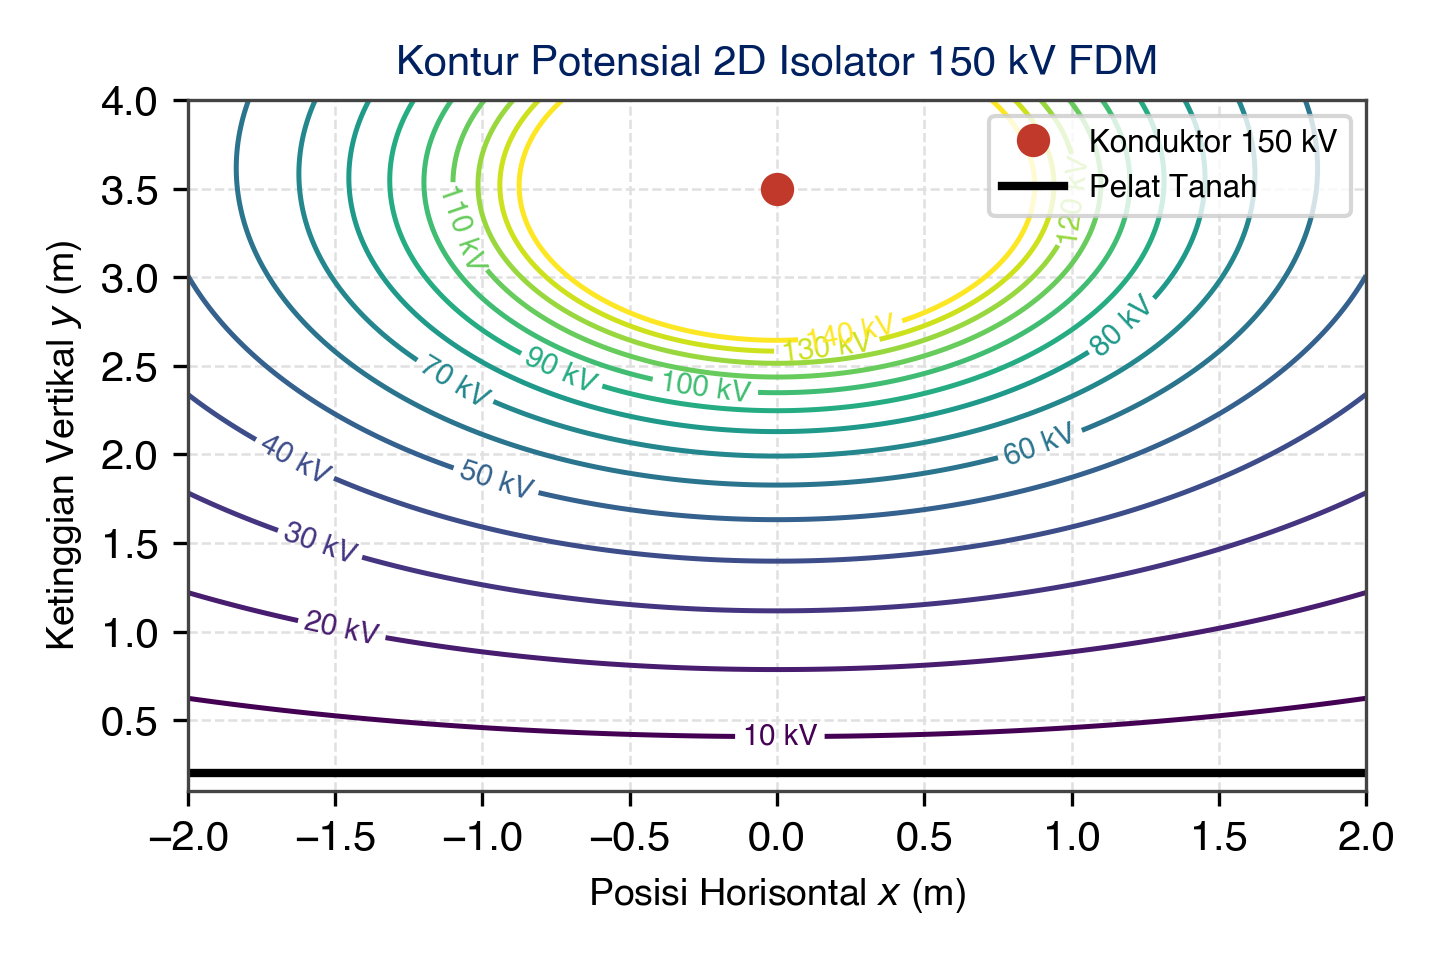
\includegraphics[width=\linewidth, height=0.38\textheight, keepaspectratio]{figures/slides/plot_ch13.png}
    \end{alertblock}
    \vspace{-0.1cm}
    \begin{exampleblock}{Intisari Medan Laplace}
      \tiny
      Kontur ekuipotensial menunjukkan kerapatan medan tertinggi ($\nabla V$) di sekitar elektroda runcing konduktor $150\text{ kV}$, mengidentifikasi titik rawan pelepasan parsial dan loncatan api (*flashover*).
    \end{exampleblock}
  \end{columns}
\end{frame}

% -------------------------------------------------------------
% FRAME 14: Kuis Tantangan Bloom Berjenjang
% -------------------------------------------------------------
% FRAME 14: Kuis & Tantangan Bloom C1-C6
\begin{frame}{Kuis Konseptual Interaktif \& Evaluasi Bloom (C1--C6)}
  \begin{columns}[t]
    \column{0.52\textwidth}
    \begin{alertblock}{Peer Instruction: Uji Miskonsepsi Fisik}
      \footnotesize
      \textbf{Kasus Rekayasa:} Teorema nilai rata-rata Gauss untuk persamaan Laplace $\nabla^2 V = 0$ membuktikan bahwa potensial di setiap titik sama dengan rata-rata sekelilingnya. Konsekuensi fisis pentingnya:
      \vspace{0.05cm}
      \begin{itemize}\setlength{\itemsep}{1pt}
        \item \textbf{[A]} Medan listrik bernilai nol di seluruh titik ruang bebas.
        \item \textbf{[B]} Potensial elektrostatika **tidak pernah memiliki titik ekstremum lokal** (maksimum/minimum selalu terletak di elektroda batas)!
        \item \textbf{[C]} Partikel bermuatan dapat melayang stabil di ruang hampa.
        \item \textbf{[D]} Kapasitansi selalu bernilai konstan independen geometri.
      \end{itemize}
    \end{alertblock}

    \column{0.46\textwidth}
    \begin{block}{Tantangan Analisis \& Desain (C4--C6)}
      \footnotesize
      \begin{itemize}\setlength{\itemsep}{2pt}
        \item \textbf{C4 (Analisis):} Buktikan Teorema Ketunggalan (*Uniqueness Theorem*) solusi persamaan Poisson/Laplace dengan identitas Green.
        \item \textbf{C5 (Evaluasi):} Evaluasi laju konvergensi metode Jacobi vs Gauss-Seidel vs Suksesif Over-Relaksasi (SOR).
        \item \textbf{C6 (Desain):} Rancang geometri cincin korona (*corona ring*) pada isolator 150 kV untuk meratakan gradien medan listrik!
      \end{itemize}
    \end{block}
  \end{columns}
\end{frame}

% -------------------------------------------------------------
% FRAME 15: Rangkuman Eksekutif & Jembatan ke Minggu 14
% -------------------------------------------------------------
\begin{frame}{Rangkuman Eksekutif \& Jembatan ke Minggu 14}
  \begin{columns}[t]
    \begin{column}{0.48\textwidth}
      \begin{block}{Rangkuman Inti Minggu 13}
        \begin{itemize}
          \item \textbf{Persamaan Laplace 2D:} Mengatur kesetimbangan elektrostatik ruang tanpa muatan ($\nabla^2 V = 0$).
          \item \textbf{Fungsi Harmonik:} Mematuhi Teorema Nilai Rata-rata Gauss dan Prinsip Ekstremum Batas.
          \item \textbf{Komputasi FDM:} Stensil 5-titik dan relaksasi cepat Successive Over-Relaxation (SOR).
          \item \textbf{Standar:} Pencegahan korona isolator tegangan tinggi sesuai \textbf{IEC 60060-1}.
        \end{itemize}
      \end{block}
    \end{column}
    \begin{column}{0.48\textwidth}
      \begin{alertblock}{Pratinjau Minggu 14: Koordinat Silindris \& Bessel}
        \begin{itemize}
          \item Bagaimana jika geometri berbentuk tabung silinder (kabel koaksial, konduktor pejal bulat)?
          \item \textbf{Persamaan Diferensial Bessel:} Muncul dari pemisahan variabel koordinat silindris $(r, \phi, z)$.
          \item Fungsi Bessel Jenis Pertama ($J_n$) dan Jenis Kedua ($Y_n$).
          \item Fenomena \textbf{Efek Kulit (\textit{Skin Effect})} frekuensi tinggi pada saluran tenaga dan telekomunikasi.
        \end{itemize}
      \end{alertblock}
    \end{column}
  \end{columns}
\end{frame}

\end{document}
